\chapter{Solutions of Non-regular Point}
\label{cha:result}
In the last chapter, we discussed various previous works in solving the non-regular point problem. However, not all these approaches are suitable for deep declarative nodes and they may not be able to optimize each parameter in the node. In this chapter, we set out to tackle solving this problem efficiently in the extension of the deep declarative network. 
\par For each scenario, we provide two practical solutions in Section~\ref{sec:overdet-sol} (overdetermined system), Section~\ref{sec:rankdf-sol} (rank deficiency problems) and Section~\ref{sec:non-convex-sol} (non-convex cases) separately. More specifically, we introduce the least-squares method and conjugate gradient preconditioning approach for the overdetermined system, which are practical and classical approximation algorithms. For rank deficient problems, we firstly propose a greedy strategy, the orthogonal matching pursuit algorithms to recover the matrix as a full rank one. We also present that in the application of the deep declarative network, how to avoid the non-regular point and minimize the approximation error. In the last scenario, we provide two theoretical methods based on the optimality conditions of the optimization problem, which are extensions of the traditional Lagrange multipliers approach. We finally prospect some future improvements for the non-regular solution in the optimization problem in Section~\ref{sec:futurework-non}. The summary of this chapter is given in the end. 

\section{Overdetermined System}
\label{sec:overdet-sol}
\subsection{Least-Squared Method}
As a classical approach to approximate the solution of the overdetermined system in linear analysis, the least-squares method is powerful and empirical in many prediction problems by minimizing the sum of the squares of the residuals.~\citep{DB:10} 
\par We begin with the linear system of equations. Supposed we have such a linear system
\begin{equation}
    \mathbf{A}\mathbf{x} = \mathbf{b}
\end{equation}
where $\mathbf{A} \in \mathbb{R}^{m \times n}$ with $m > n$, $\mathbf{x} \in \mathbb{R}^n$ and $\mathbf{b} \in \mathbb{R}^{m}$. Therefore, there are more equations than unknowns, which is an overdetermined system and there is no solution making $\mathbf{A}\mathbf{x} = \mathbf{b}$ for all $\mathbf{x}$. $\mathbf{b}$ is also not in the column subspace of $\mathbf{A}$, hence $\mathbf{b}$ is actually not a linear combination of the column vectors of $\mathbf{A}$. With the least-square method, we want to find an $\mathbf{x}$ which makes the residual vector $\mathbf{r} \in \mathbb{R}^m$ approaching zero:
\begin{equation}
    \label{equ:residual}
    \mathbf{r} = \mathbf{b} - \mathbf{A}\mathbf{x}, \text{for each element in } \mathbf{r}:  r_i = b_i - \sum_{j=1}^{n} a_{i j} x_{j}, \quad i = 1, \dots, m
\end{equation}
\par The solution $\mathbf{x}$ in Equation~\ref{equ:residual} given be the least squares method minimizes $\|\mathbf{r}\|_2 = \|\mathbf{b} - \mathbf{A}\mathbf{x}\|_2$, which is also the sum of errors:
\begin{equation}
    \label{equ:lstsq}
    \|\mathbf{r}\|_2 = \mathbf{r}^{T} \mathbf{r}=(\mathbf{b}-\mathbf{A} \mathbf{x})^{T}(\mathbf{b}-\mathbf{A} \mathbf{x})=\mathbf{b}^{T} \mathbf{b}-\mathbf{x}^{T} \mathbf{A}^{T} \mathbf{b}-\mathbf{b}^{T} \mathbf{A} \mathbf{x}+\mathbf{x}^{T} \mathbf{A}^{T} \mathbf{A} \mathbf{x}
\end{equation}
\par We aim to find the optimal approximation $\mathbf{x}$ that minimize the $\|\mathbf{r}\|_2$ in Equation~\ref{equ:lstsq}. Therefore, we compute the derivative of Equation~\ref{equ:lstsq} with respect to $x_k, k = 1, \dots, n$ and set it equal to zero
\begin{equation}
    \label{equ:lstsq-gradient}
    \frac{\partial \|\mathbf{r}\|}{\partial x_{k}}=\frac{\partial}{\partial x_{k}}\left[\sum_{i=1}^{m}\left(b_{i}-\sum_{j=1}^{n} a_{i j} x_{j}\right)^{2}\right]=2 \sum_{i=1}^{m}\left(b_{i}-\sum_{j=1}^{n} a_{i j} x_{j}\right)\left(-a_{i k}\right)=0)
\end{equation}
where $a_{ij}$ are elements in $\mathbf{A}$. 
\par From Equation~\ref{equ:lstsq-gradient}, we can find
\begin{equation}
    \sum_{i=1}^{m} \sum_{j=1}^{n} a_{i j} a_{i k} x_{j}=\sum_{j=1}^{n}\left[\sum_{i=1}^{m} a_{i j} a_{i k}\right] x_{j}=\sum_{i=1}^{m} b_{i} a_{i k}
\end{equation}
which is equivalent to
\begin{equation}
    \mathbf{A}^{T} \mathbf{A} \mathbf{x}=\mathbf{A}^{T} \mathbf{b}
\end{equation}
\par Consequently, we can solve $\mathbf{x}$
\begin{equation}
    \mathbf{x}=\left(\mathbf{A}^{T} \mathbf{A}\right)^{-1} \mathbf{A}^{T} \mathbf{b}=\mathbf{A}^{-} \mathbf{b}
\end{equation}
where $\mathbf{A}^{-}$ is the pseudoinverses of $\mathbf{A}$ and $\mathbf{A}^{T} \mathbf{A}$ is supposed to be invertible since $\operatorname{rank}\mathbf{A} < \operatorname{min}(m, n)$.
\begin{figure}[t]
    \label{fig:least-square}
    \centering
    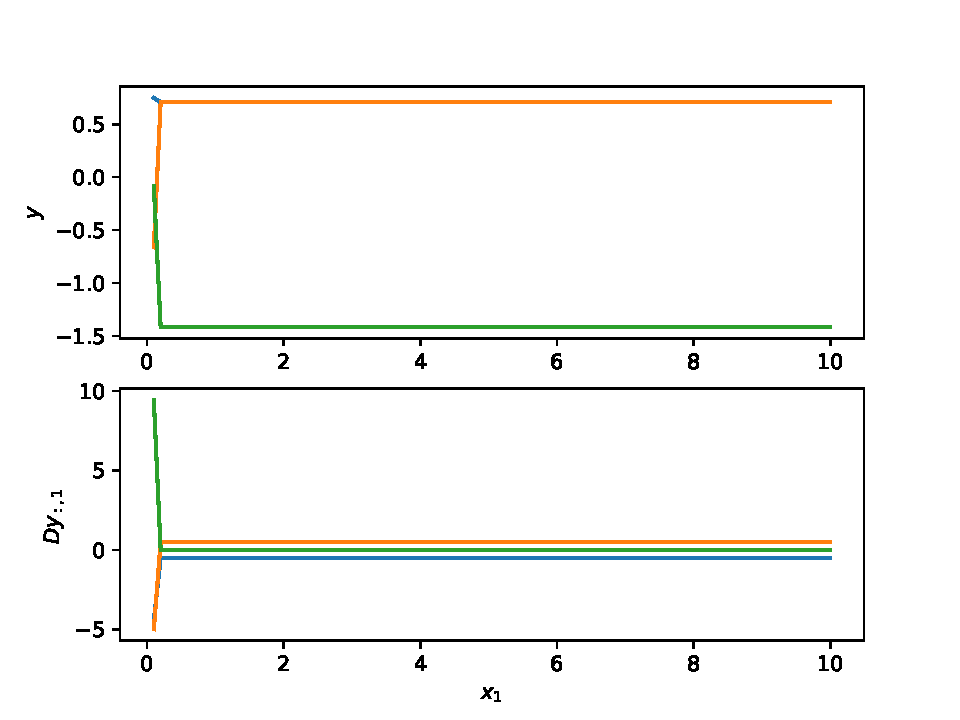
\includegraphics[page=1, width=.8\textwidth]{figs/least-square.pdf}
    \caption{Plots of the function $y$ (top) and the gradient (bottom) sweeping the first component of the input $x_1$ while holding the other elements of $x$ constant with the least-squares method}
\end{figure}
\par In deep declarative nodes, if constraints are not second-order differentiable, matrix $B=\mathrm{D}_{X Y}^{2} f(x, y)-\sum_{i=1}^{p+q} \lambda_{i} \mathrm{D}_{X Y}^{2} \tilde{h}_{i}(x, y) \in \mathbb{R}^{m \times n}$ and matrix $H=\mathrm{D}_{Y Y}^{2} f(x, y)-\sum_{i=1}^{p+q} \lambda_{i} \mathrm{D}_{Y Y}^{2} \tilde{h}_{i}(x, y) \in \mathbb{R}^{m \times m}$ are undefined. Therefore, there is no exact solution for the linear system $Hx_1 = A^T$ and $Hx_2 = B$ since it is overdetermined. In this circumstance, using the least-squares method to approximate the solution of the linear system is a classical approach. Figure~\ref{fig:least-square} shows an example of overdetermined system using the least-squares method to approximate the solution of the gradient, where the gradient in one of three variables converges to zero and others are almost zero. 
\par The least-squares method is very basic and practical since the residual between the ground truth and approximation is minimized, which usually leads the optimal solution. Many methods are based on this in solving different non-regular solution problems, which will be discussed in Section~\ref{sec:rankdf-sol} and Section~\ref{sec:non-convex-sol}. 

\subsection{Conjugate Gradient and Preconditioning}
We mentioned the steepest method in solving unconstrained optimization problems in Section~\ref{sec:consopt}. In general, the steepest gradient descent takes several steps in the same direction. In the conjugate gradient method, it only takes one step in each direction from a set of orthogonal search directions~\citep{HM:52}.
\par Supposed we have such a set of orthogonal search directions $\mathbf{d}_{(0)}, \mathbf{d}_{(1)}, \cdots, \mathbf{d}_{(n-1)}$, and we update the gradient $\mathbf{x}$ $n$ steps
\begin{equation}
    \label{equ:update-graident}
    \mathbf{x}_{(i+1)}=\mathbf{x}_{(i)}+\alpha_{(i)} \mathbf{d}_{(i)}
\end{equation}

where $\alpha_i$ is the step size. To determine the value of $alpha_i$ for each movement under the orthogonal relation between the residual $\mathbf{e}_{(i+1)}$ and the gradient direction $\mathbf{d}_{(i)}$, we take different direction for each update
\begin{equation}
    \begin{aligned} 
        \mathbf{d}_{(i)}^{T} \mathbf{e}_{(i+1)} &=0 \\ \mathbf{d}_{(i)}^{T}\left(\mathbf{e}_{(i)}+\alpha_{(i)} \mathbf{d}_{(i)}\right) &=0 \\ \alpha_{(i)} &=-\frac{\mathbf{d}_{(i)}^{T} \mathbf{e}_{(i)}}{\mathbf{d}_{(i)}^{T} \mathbf{d}_{(i)}} 
    \end{aligned}
\end{equation}
where the residual $\mathbf{e}_{(i+1)}$ is the difference between the ground truth $x$ and the current updated $\mathbf{x}_{i+1}$. 
\begin{figure}[t]
    \label{fig:ortho-gradient}
    \centering
    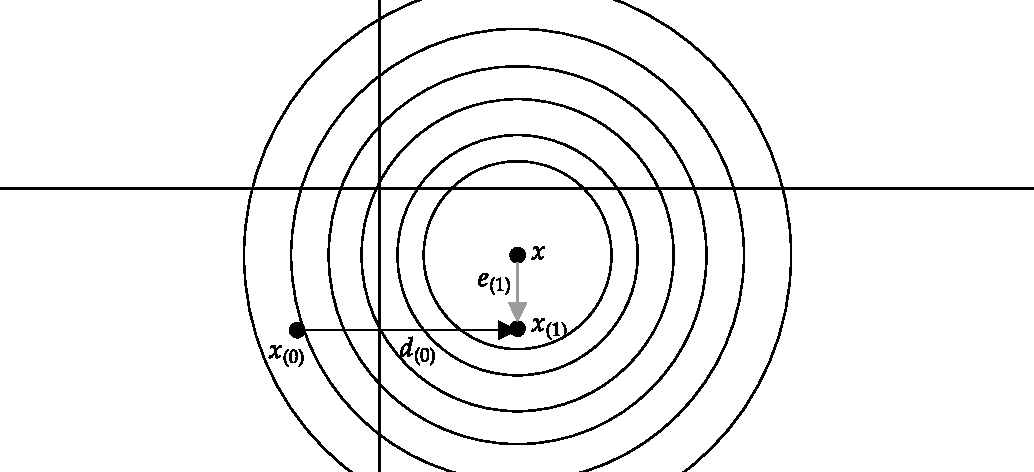
\includegraphics[page=1, width=.8\textwidth]{figs/orthogonal-gradient.pdf}
    \caption{Directions of the orthogonal gradient method}
\end{figure}
\par Figure~\ref{fig:ortho-gradient} shows the gradient update from $x_{(0)}$ to $x_{1}$ using the orthogonal gradient method, where $x$ is the ground truth and $x_{(1)}$ is the updated gradient. From this figure, it is clear that the direction of vector $d_{(0)}$ and the residual vector $e_{(1)}$ are orthogonal. However, we cannot decide the $\mathbf{e}_{(i)}$, so we used to make these two vectors $\mathbf{A}$-orothogonal, which means
\begin{equation}
    \label{equ:a-otho}
    \left\langle\mathbf{d}_{(i)}, \mathbf{e}_{(i+1)}\right\rangle_{A}:=\mathbf{d}_{(i)}^{T} \mathbf{A} \mathbf{e}_{(i+1)}=0
\end{equation}
\begin{figure}[t]
    \label{fig:a-ortho}
    \centering
    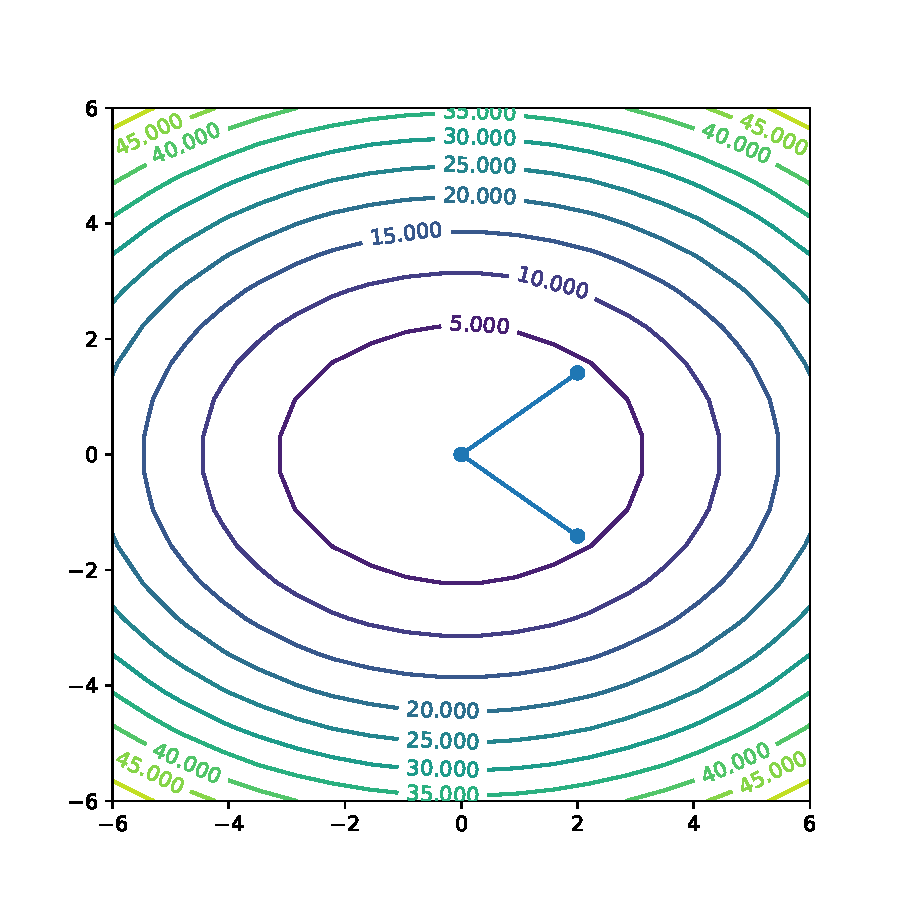
\includegraphics[page=1, width=.6\textwidth]{figs/a-orthogonal-example.pdf}
    \caption{$A$-orthogonality between two vectors}
\end{figure}
\par Figure~\ref{fig:a-ortho} is an example of the $A$-orthogonality between two vectors. They are not exactly orthogonal, but $A$-orthogonal. 
\par From the Equation~\ref{equ:a-otho}, we get the step size
\begin{equation}
    \label{equ:ini-stepsize}
    \alpha_{(i)}=\frac{\mathbf{d}_{(i)}^{T} \mathbf{r}_{(i)}}{\mathbf{d}_{(i)}^{T} \mathbf{A} \mathbf{d}_{(i)}}
\end{equation}
where in this case, the two vectors are not absolutely orthogonal and it depends on the matrix $\mathbf{A}$. This $\mathbf{A}$-orthogonality is applied to the direction set $\left\{\mathbf{d}_{(i)}\right\}$. We decide the search directions through $n$ linearly independent vectors $\mathbf{u}$
\begin{equation}
    \mathbf{d}_{(i)}=\mathbf{u}_{i}+\sum_{k=0}^{i-1} \beta_{i, k} \mathbf{d}_{(k)}, \quad i>0
\end{equation}
where 
\begin{equation}
    \label{equ:update-beta}
    \beta_{i, j}=\frac{-\mathbf{u}_{i}^{T} \mathbf{A} \mathbf{d}_{(j)}}{\mathbf{d}_{(j)}^{T} \mathbf{A} \mathbf{d}_{(j)}}
\end{equation}
which the second direction based on the $\mathbf{A}$-orthogonality. 
\par Now from above theorems, we can choose the conjugate directions which are constructed by conjugation of the residuals. Since the residuals are orthogonal to the previous search directions, it is graranteed to produce a new linearly independent search direction, until the residual is zero. Therefore, we only need to keep the previous search direction each time to update the gradient. 
\begin{figure}[t]
    \label{fig:conj-gradient}
    \centering
    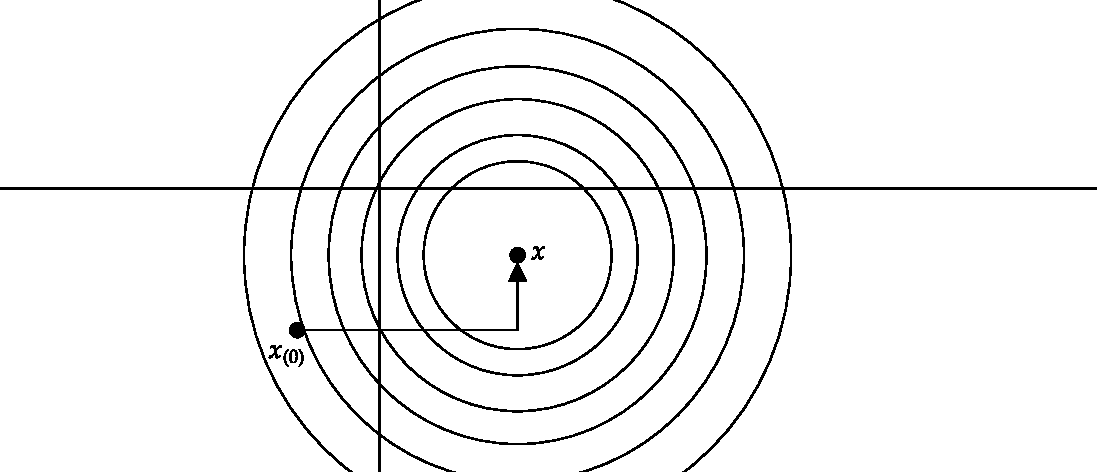
\includegraphics[page=1, width=.6\textwidth]{figs/conjugate-gradient.pdf}
    \caption{Conjugate gradient method}
\end{figure}
\par The completed conjugate gradient method can be concluded as follows:
\begin{itemize}
    \item Decide first conjugate direction $\mathbf{d}_{(0)}:=\mathbf{u}_{(0)}=\mathbf{b}-\mathbf{A} \mathbf{x}_{(0)}$ from the linear system.
    \item Calculate the step size based on the $\mathbf{A}$-orthogonality from Equation~\ref{equ:ini-stepsize}.
    \item Update the gradient from Equation~\ref{equ:update-graident}.
    \item Update the set of linearly independent vectors $\mathbf{u}_{(i+1)}:=\mathbf{u}_{(i)}-\alpha_{(i)} \mathbf{A} \mathbf{d}_{(i)}$
    \item Calculate the current step size $\beta$ based on the previous one $\alpha$ through Equation~\ref{equ:update-beta}. 
    \item Calculate the next conjugate direction based on the new linearly independent vectors, the current step size, and the previous conjugate direction:
    $$
    \mathbf{d}_{(i+1)}:=\mathbf{u}_{(i+1)}+\beta_{(i+1)} \mathbf{d}_{(i)}
    $$
\end{itemize}
\par Figure~\ref{fig:conj-gradient} shows a simple example of the conjugate gradient method, which achieves the ground truth with two steps. 
\par Obviously, for overdetermined linear systems, the traditional conjugate gradient method does not work. We introduce the method of preconditioning~\cite{SJ:94} to solve $\mathbf{A}\mathbf{x}=\mathbf{b}$ indirectly. In the preconditioning method, it demonstrates a positive definite invertible preconditioner $\mathbf{M}$ as the approximation of $\mathbf{A}$, which can convert the problem to solving 
\begin{equation}
    \mathbf{M}^{-1} \mathbf{A} \mathbf{x}=\mathbf{M}^{-1} \mathbf{b}
\end{equation}
where $\mathbf{M}^{-1} \mathbf{A}$ is usually not symmetric. Hence, matrix decomposition $\mathbf{E} \mathbf{E}^{T}=\mathbf{M}$ is performed to transform the problem as $\mathbf{M}^{-1} \mathbf{A}$ and $\mathbf{E}^{-1} \mathbf{A} \mathbf{E}^{-T}$ share the same eigenvalues
\begin{equation}
    \label{equ:pre-conj-linear-sys}
    \mathbf{E}^{-1} \mathbf{A} \mathbf{E}^{-T} \hat{\mathbf{x}}=\mathbf{E}^{-1} \mathbf{b} \quad \hat{\mathbf{x}}=\mathbf{E}^{T} \mathbf{x}
\end{equation}
\par Combining the result of the linear system in Equation~\ref{equ:pre-conj-linear-sys} and the conjugate gradient method, we get this transformed conjugate gradient method~\citep{SJ:94}. The choices of the preconditioner are various. The perfect one is that $\mathbf{M} := \mathbf{A}$ but it is not anymore useful. The diagonal preconditioner, which is easy to calculate in finding a solution, is also a reasonable choice. Another preconditioner is the incomplete Cholesky factor, turning $\mathbf{A} = \mathbf{L}\mathbf{L}^T$ with partial Gaussian elimination. 
\par Using the transformed conjugate gradient method to solve linear systems helps to approximate the solution of the overdetermined system. In deep declarative nodes, we can adopt this approach to solve the linear system $Hx_1 = A^T$ and $Hx_2 = B$ iteratively. Comparing with the least-squares method, the preconditioned conjugate gradient method is not so direct since it takes iterations to converge. However, it can be more stable to get the ideal approximation. 


\section{Rank Deficiency}
\label{sec:rankdf-sol}
\subsection{Orthogonal Matching Pursuit Algorithm}
Rank deficiency is also known as the underdetermined system, which means the system has less equations than the unknowns. In a linear system $Ax=b$, if $A$ is rank deficient, there are two problems. The first problem is that there is not be an exact solution at all. Since the range of $A$ does not span the entire $\mathbb{R}^n$ (if $A$ has $n$ columns) but only an $(N-1)$-dimensional subspace. In this case, we can solve exactly for $x$ only if $b$ is in this subspace. The second problem is that there are actually infinity solutions, since $A$ has a non-empty null space, which means that there is a 1-dimensional subspace of vectors $x$ that gives $Ax=0$. If we use the least-squares solution, the pseudoinverses of $A$ multiply by $b$, it provides a solution for both problems. For the first problem, it gives the closest $x$, which is also the one with the smallest $\|b-Ax\|$. At the same time, for the second problem, out of all solutions that share the smallest approximation error and it gives the one with the smallest norm, which is the minimum-norm solution. Therefore, applying the least-squares method to rank deficient may not be able to obtain the best solution for all columns in the matrix. 
\par We consider the orthogonal matching pursuit algorithm (OMP), which is a greedy compressed approach widely used in signal recovery~\citep{MS:93}. The goal of this algorithm is to recover the sparse signal vectors from a small number of measurements. Supposed we consider a $K$-sparse signal vector $\mathbf{x}$, which is an $n$-dimensional vector with at most $K$ non-zero elements, transformed into a smaller $m$-dimensional $\mathbf{y}$ based on matrix $\mathbf{\Phi}$
\begin{equation}
    \label{equ:signal-recover}
    \mathbf{y}=\mathbf{\Phi} \mathbf{x}
\end{equation}
\par In compressive sensing, we use to set $n > m$. Therefore, the system of Equation~\ref{equ:signal-recover} is underdetermined and the matrix $\mathbf{\Phi}$ is rank deficient. Also, there is no exact solution can be obtained. The OMP algorithm provides a simple but competitive solution for solving this underdetermined system by selecting the best fitting column of the sensing matrix iteratively. Besides, a least-squares optimization is performed in the subspace spanned by all previously picked columns. 
\par We give the details of the OMP algorithm with the classical linear system $Ax = b$ where $A \in \mathbb{R}^{m \times n}, b \in \mathbb{R}^{m}$. An optional operation before the OMP iteration is the normalization of columns in the matrix $A$, which transforms them into unit vectors
\begin{equation}
    a_{i} \leftarrow \frac{a_{i}}{\left\|a_{i}\right\|_{2}}
\end{equation}
where $a_i$ are the columns of $A$. This normalization step is to make sure any correlations between two columns of $A$ within the range $[-1, 1]$, which also bound the absolute value within 1. 


\subsection{Strategies in Applications}

\section{Non-convex Problems}
\label{sec:non-convex-sol}
\subsection{Augumented Lagrange Method}
\subsection{Non-linear Lagrangian Duality}



\section{Future Work of the Solution for Non-regular Points}
\label{sec:futurework-non}


\section{Summary}
